\documentclass{nada-ten}
\usepackage[utf8]{inputenc}
\usepackage[swedish,english]{babel}
\usepackage{array}
%\usepackage{qbordermatrix}
\usepackage{graphicx}
\graphicspath{{figures/}}
\usepackage{upquote} % this is to make straight apostrophes in verbatim
\usepackage{listings}

\usepackage{tipa}

\author{Giampiero Salvi}
\course{DT2119 Speech and Speaker Recognition}
\semester{Vårterminen \the\year}
\title{DT2119 Lab1: Feature extraction}

\begin{document}
\maketitle
%\setlanguage{english}
\section{Objective}
The objective is to experiment with different features commonly used for speech analysis and recognition. The lab is designed in Python, but the same functions can be obtained in Matlab/Octave or using the Hidden Markov Toolkit (HTK). In Appendix~\ref{sec:appendix}, a reference table is given indicating the correspondence between different systems.

\section{Task}

\begin{itemize}
\item compute Mel Filterbank and MFCC features step-by-step
\item examine features
\item evaluate correlation between feature
\item compare utterances with Dynamic Time Warping
\item illustrate the discriminative power of the features with respect to words
\item perform hierarchical clustering of utterances
\item train and analyze a Gaussian Mixture Model of the feature vectors.
\end{itemize}

In order to pass the lab, you will need to follow the steps described in this document, and present your results to a teaching assistant. Use Canvas to book a time slot for the presentation. Remember that the goal is not to show your code, but rather to show that you have understood all the steps.

\paragraph{Note for VT2020:}
Because of the current quarantine situation, it is recommended that you use one of the cloud services (for example Google Colab\footnote{\url{https://colab.research.google.com}}) and solve the exercise in a shared notebook.

%\section{Preliminaries}
%\subsection{Python Instructions}
%If you use python, you can refer to the \verb|scikits.talkbox| as a reference to the feature extraction functions. Use the \verb|python setup.py install --user| command if you do not have rights to install packages as administrator.

%\subsection{Spectral content in speech}
%The file \verb|speech48kHz.wav| contains a single channel recording of a few sentences sampled at 48kHz, 16 bits linear coding. Use Wavesurfer\footnote{\url{http://sourceforge.net/projects/wavesurfer/}} to open and listen to the files. Create a Waveform and a Spectrogram pane. Observe the distribution of energy in time and frequency. Use the Spectrogram Controls to increase the Analysis window length to the maximum value. Select the whole speech file and use the LTAS function to compute the Long Time Average Spectrum.

%Resample the file with Sox\footnote{\url{http://sox.sourceforge.net/} In Ubuntu \texttt{sudo apt-get install sox}} (command \verb|rate -v |) to 16kHz and 8kHz. Compare the 48, 16 and 8kHz versions with Wavesurfer. Is the speech as intelligible in each of the files? Do you hear any difference in quality?
%Open the file in Python (consult the \verb|scipy.io.wavfile| module). Resample the speech to 16kHz and 8kHz using
% \verb|scipy.signal.resample|
% \verb|scikits.samplerate|\footnote{on Ubuntu you will need the package \verb|libsamplerate0-dev| in order to install the python package}. Compare the 48, 16 and 8kHz versions with Wavesurfer. Is the speech as intelligible in each of the files? Do you hear any difference in quality?
%Resample the 48kHz file to 16kHz and 8kHz by hand by just keeping every third or fourth sample. Is there any difference from the results obtained with \verb|scipy.signal.resample|? In case, what do you think this depends on?

\section{Data}
The files \verb|lab1_data.npz| and \verb|lab1_example.npz| contain the data to be used for this exercise.
%\footnote{Note on Python 3: the file formats between Python 2 and 3 are not compatible. If you use version 3, use the file \texttt{tidigits\_python3.npz} and \texttt{example\_python3.npz}, instead.}.
The files contains two arrays: \texttt{data} and \texttt{example}\footnote{If you wish to use Matlab/Octave instead of Python, use the provided \texttt{py2mat.py} script to convert to Matlab format. Load the file with \texttt{load lab1\_data} or \texttt{lab1\_example}. You will load two cell arrays with the corresponding data stored in structures.}.

\subsection{example}
The array \texttt{example} can be used for debugging because it contains calculations of all the steps in Section~\ref{sec:mfcc} for one utterance. It can be loaded with:
\begin{verbatim}
import numpy as np
example = np.load('lab1_example.npz', allow_pickle=True)['example'].item()
\end{verbatim}

The element \texttt{example} is a dictionary with the following keys:

\vspace{2mm}
\begin{tabular}{ll}
  \texttt{samples}: & speech samples for one utterance \\
  \texttt{samplingrate}: & sampling rate \\
  \texttt{frames}: & speech samples organized in overlapping frames \\
  \texttt{preemph}: & pre-emphasized speech samples \\
  \texttt{windowed}: & hamming windowed speech samples \\
  \texttt{spec}: & squared absolute value of Fast Fourier Transform \\
  \texttt{mspec}:   & natural log of \texttt{spec} multiplied by Mel filterbank \\
  \texttt{mfcc}:    & Mel Frequency Cepstrum Coefficients \\
  \texttt{lmfcc}:   & Liftered Mel Frequency Cepstrum Coefficients
\end{tabular}
\vspace{2mm}

Figure~\ref{fig:mfcc} shows the content of the elements in \texttt{example}.
\begin{figure}
  \centering
  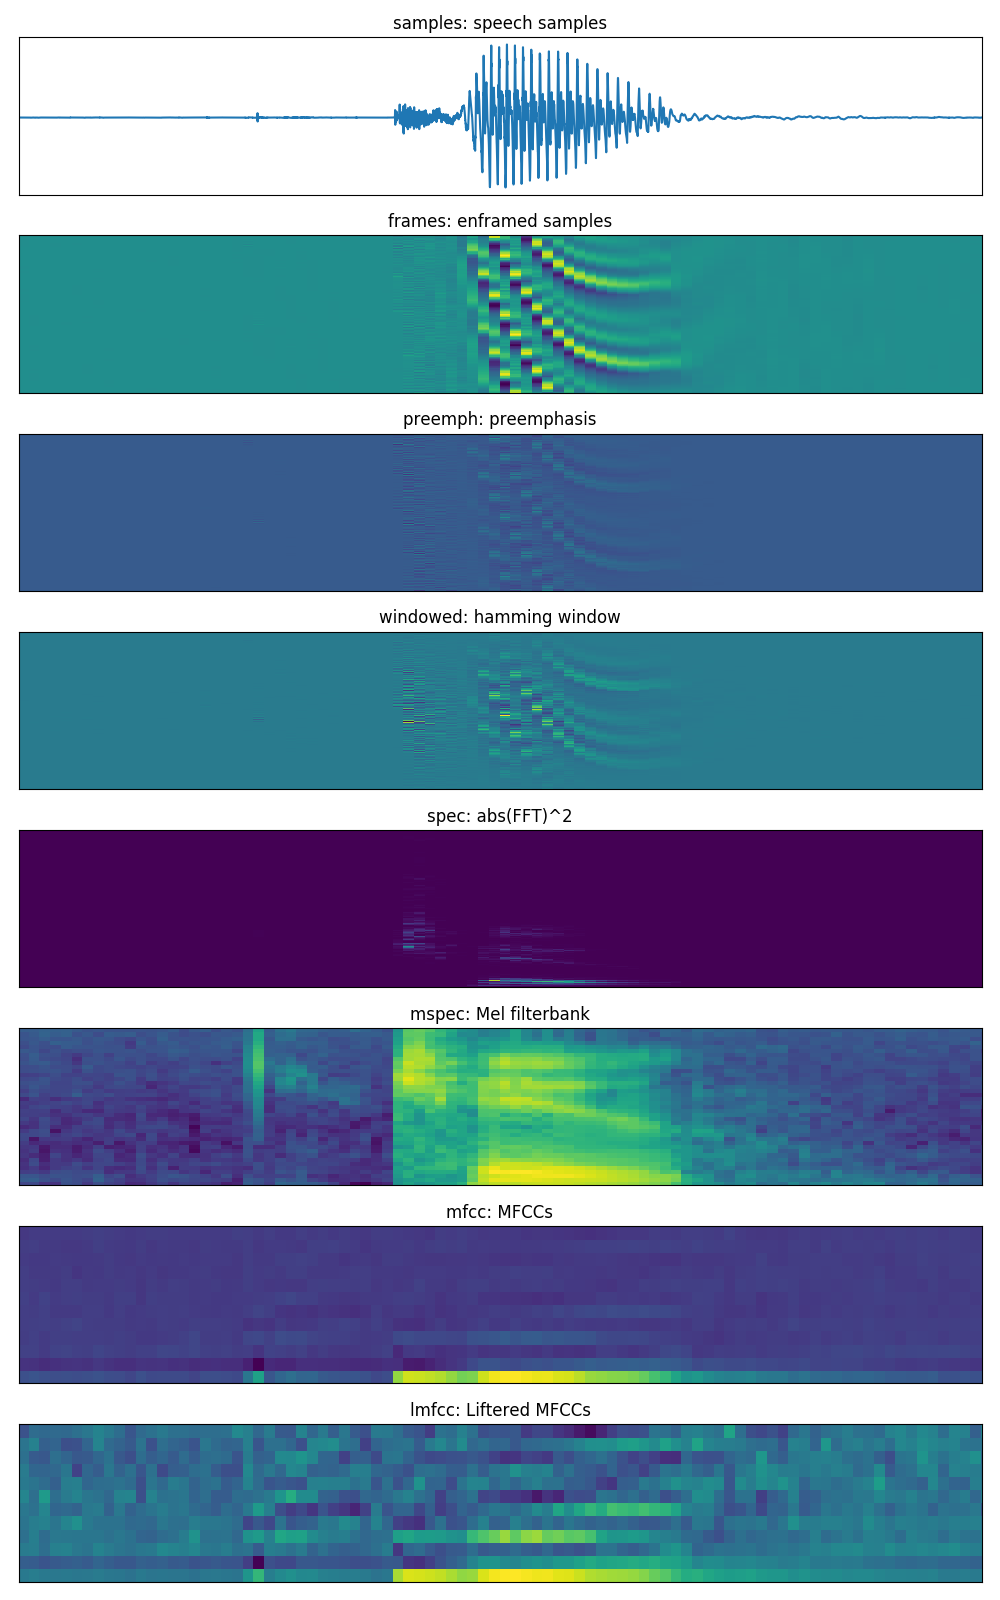
\includegraphics[width=0.8\textwidth]{MFCC_step_by_step}
  \caption{Evaluation of MFCCs step-by-step}
  \label{fig:mfcc}
\end{figure}

\subsection{data}
The array \texttt{data} contains a small subset of the TIDIGITS database (\url{https://catalog.ldc.upenn.edu/LDC93S10}) consisting of a total of 44 spoken utterances from one male and one female speaker\footnote{The complete database contains recordings from 225 speakers}. The file was generated with the script \verb|lab1_data.py|\footnote{The script is included only for reference in case you need to use the full database in the future. In that case, you will need access to the KTH AFS file system.}. For each speaker, 22 speech files are included containing two repetitions of isolated digits (eleven words: ``oh'', ``zero'', ``one'', ``two'', ``three'', ``four'', ``five'', ``six'', ``seven'', ``eight'', ``nine''). You can read the file from Python with:
\begin{verbatim}
data = np.load('lab1_data.npz', allow_pickle=True)['data']
\end{verbatim}
The variable \verb|data| is an array of dictionaries. Each element contains the following keys:

\begin{tabular}{ll}
  \verb|filename|: & filename of the wave file in the database \\
  \verb|samplingrate|: & sampling rate of the speech signal (20kHz in all examples) \\
  \verb|gender|: & gender of the speaker for the current utterance (\texttt{man}, \texttt{woman}) \\
  \verb|speaker|: & speaker ID for the current utterance (\texttt{ae}, \texttt{ac})\\
  \verb|digit|: & digit contained in the current utterance (\texttt{o, z, 1, \dots, 9})\\
  \verb|repetition|: & whether this was the first (\texttt{a}) or second (\texttt{b}) repetition \\
  %\verb|wid|: & word id summarizing gender, speaker, digit and repetition (e.g. \texttt{man\_ae\_3\_b}) \\
  \verb|samples|: & array of speech samples
\end{tabular}

\section{Mel Frequency Cepstrum Coefficients step-by-step}
\label{sec:mfcc}
Follow the steps below to computer MFCCs. Use the \texttt{example} array to double check that your calculations are right.

You need to implement the functions specified by the headers in \texttt{lab1\_proto.py}. Once you have done this, you can use the function \texttt{mfcc} in \texttt{lab1\_tools.py} to compute MFCC coefficients in one go.
%\lstset{showstringspaces=false}

\subsection{Enframe}
Implement the \texttt{enframe} function in \texttt{lab1\_proto.py}. This will take as input speech samples, the frame length in samples and the number of samples overlap between consecutive frames and outputs a two dimensional array where each row is a frame of samples. Consider only the frames that fit into the original signal disregarding extra samples. Apply the enframe function to the utterance \verb|example['samples']| with window length of 20 milliseconds and shift of 10 ms (figure out the length and shift in samples from the sampling rate). Use the \texttt{pcolormesh} function from \texttt{matplotlib.pyplot} to plot the resulting array.
%(use the options \verb|origin='lower'|, \verb|interpolation='nearest'| and \verb|aspect='auto'| in order to produce similar plots to Figure~\ref{fig:mfcc}).
Verify that your result corresponds to the array in \verb|example['frames']|.

\subsection{Pre-emphasis}
Implement the \texttt{preemp} function in \texttt{lab1\_proto.py}. To do this, define a pre-emphasis filter with pre-emphasis coefficient 0.97 using the \texttt{lfilter} function from \verb|scipy.signal|. Explain how you defined the filter coefficients. Apply the filter to each frame in the output from the \verb|enframe| function. This should correspond to the \verb|example['preemph']| array.

\subsection{Hamming Window}
Implement the \texttt{windowing} function in \texttt{lab1\_proto.py}. To do this, define a hamming window of the correct size using the \texttt{hamming} function from \verb|scipy.signal| with extra option \texttt{sym=False}\footnote{The meaning of this option is beyond the scope of this course, but you should use it if you want to get the same results as in the example.}. Plot the window shape and explain why this windowing should be applied to the frames of speech signal. Apply hamming window to the pre-emphasized frames of the previous step. This should correspond to the \verb|example['windowed']| array.

\subsection{Fast Fourier Transform}
Implement the \texttt{powerSpectrum} function in \texttt{lab1\_proto.py}. To do this, compute the Fast Fourier Transform (FFT) of the input from \verb|scipy.fftpack| and then the squared modulus of the result. Apply your function to the windowed speech frames, with FFT length of 512 samples. Plot the resulting power spectrogram with \texttt{pcolormesh}. Beware of the fact that the FFT bins correspond to frequencies that go from 0 to $f_{\mbox{max}}$ and back to 0. What is $f_{\mbox{max}}$ in this case according to the Sampling Theorem? The array should correspond to \verb|example['spec']|.
%\lstinputlisting[language=Python]{../prototypes/lab1\_tools.py}

\subsection{Mel filterbank log spectrum}
Implement the \texttt{logMelSpectrum} function in \texttt{lab1\_proto.py}. Use the \verb|trfbank| function, provided in the \texttt{lab1\_tools.py} file, to create a bank of triangular filters linearly spaced in the Mel frequency scale. Plot the filters in linear frequency scale. Describe the distribution of the filters along the frequency axis. Apply the filters to the output of the power spectrum from the previous step for each frame and take the natural log of the result. Plot the resulting filterbank outputs with \texttt{pcolormesh}. This should correspond to the \verb|example['mspec']| array.

\subsection{Cosine Transofrm and Liftering}
Implement the \texttt{cepstrum} function in \texttt{lab1\_proto.py}. To do this, apply the Discrete Cosine Transform (\texttt{dct} function from \verb|scipy.fftpack.realtransforms|) to the outputs of the filterbank. Use coefficients from 0 to 12 (13 coefficients). Note that using the \texttt{n=13} input parameter in \texttt{dct} is not the same as running without the argument and taking the first 13 elements in the results, try to explain why.  Then apply liftering using the function \verb|lifter| in \texttt{lab1\_tools.py}. This last step is used to correct the range of the coefficients. Plot the resulting coefficients with \texttt{pcolormesh}. These should correspond to \verb|example['mfcc']| and \verb|example['lmfcc']| respectively.

Once you are sure all the above steps are correct, use the \texttt{mfcc} function (\texttt{lab1\_proto.py}) to compute the liftered MFCCs for all the utterances in the \texttt{data} array. Observe differences for different utterances.

\section{Feature Correlation}
Concatenate all the MFCC frames from all utterances in the \texttt{data} array into a big feature $[N \times M]$ array where $N$ is the total number of frames in the data set and $M$ is the number of coefficients. Then compute the correlation coefficients between features\footnote{Note that we want the correlation between feature coefficients, and not between consecutive feature vectors, that is the resulting correlation matrix should be $M\times M$.} and display the result with \texttt{pcolormesh}. Are features correlated? Is the assumption of diagonal covariance matrices for Gaussian modelling justified? Compare the results you obtain for the MFCC features with those obtained with the Mel filterbank features (\verb|'mspec'| features).

% \section{Gaussian Mixture Models}
% Use the concatenated MFCCs from the previous section to train a Gaussian Mixture Model with the class \texttt{GMM} from \texttt{sklearn.mixture}. Use 16 components for the mixture with diagonal covariance matrices. For each utterance in the \texttt{data} array and using the trained model, compute posterior probabilities per frame and Gaussian in the model. Display the probabilities for some utterance.

\section{Explore Speech Segments with Clustering}

Using the concatenated data from the previous section, train a Gaussian mixture model with \texttt{sklearn.mixture.GMM} (or \texttt{sklearn.mixture.GaussianMixture} depending on the version of \texttt{sklearn}).
Vary the number of components for example: 4, 8, 16, 32.
Once the models are trained, compute GMM posteriors for utterances containing the same words.
Plot the results with \texttt{pcolormesh} and observe the evolution of the GMM posteriors in time.
\begin{itemize}
\item Can you say something about the classes discovered by the unsupervised learning method?
\item Do the classes roughly correspond to the phonemes you expect to compose each word?
\item Are those classes a stable representation of the word if you compare utterances from different speakers.
\end{itemize}
As an example, plot and discuss the GMM posteriors for the model with 32 components for the four occurrences of the word ``seven'' (utterances 16, 17, 38, and 39).

\section{Comparing Utterances}
Given two utterances of length $N$ and $M$ respectively, compute an $[N\times M]$ matrix of local Euclidean distances between each MFCC vector in the first utterance and each MFCC vector in the second utterance.

Write a function called \texttt{dtw} (\texttt{lab1\_proto.py}) that takes as input this matrix of local distances and outputs the result of the Dynamic Time Warping algorithm. The main output is the global distance between the two sequences (utterances), but you may want to output also the best path for debugging reasons.

For each pair of utterances in the  \texttt{data} array:
\begin{enumerate}
\item compute the local Euclidean distances between MFCC vectors in the first and second utterance
\item compute the global distance between utterances with the \texttt{dtw} function you have written
\end{enumerate}
Store the global pairwise distances in a matrix $D$ ($44\times 44$). Display the matrix with \texttt{pcolormesh}. Compare distances within the same digit and across different digits. Does the distance separate digits well even between different speakers?

Run hierarchical clustering on the distance matrix $D$ using the \texttt{linkage} function from
\texttt{scipy.cluster.hierarchy}. Use the ''complete'' linkage method. Display the results with the function \texttt{dendrogram} from the same library, and comment them. Use the \texttt{tidigit2labels} function (\texttt{lab1\_tools.py}) to create labels to add to the dendrogram to simplify the interpretation of the results.

%Repeat the same procedure using standardized data, that is remove the global mean and divide by the global standard deviation of the MFCCs. Does this improve results? Also try using GMM posteriors as features instead of MFCCs. Do you notice any difference?

% Here the task is to study the correlation between coefficients in a particular representation on large sets of data. A simple way to extract feature vectors across many audio files when the labels are not required is by using the Unix command \verb|find|:
% \begin{verbatim}
% find data/ -name "TR*.wav" -exec HList -C features_MFCC_0.cfg -r {} \; | \
%        gzip > /tmp/mfcc_0.txt.gz
% \end{verbatim}
% This command will do the following:
% \begin{enumerate}
% \item find all files under the directory \verb|data| with name matching the pattern \verb|TR*.wav|
% \item for each file found, execute the HList command which extracts the features according to the parameters in the configuration file and outputs them to standard output in ascii format
% \item concatenate all results and zip them
% \item save the zipped data into the file specified by the last term
% \end{enumerate}
% If you are not using a Posix system such as Linux, Unix or Mac OS X, you will have find a way to execute \verb|HList| on all the files and then to collect the results into a single text file.

% Now you can safely load the gzipped file in Octave with the standard \verb|load| function, into a variable that will contain an $N\times M$ matrix, where $N$ is the number of feature vectors and $M$ is the number of coefficients per vector (dimensionality of the representation). $N$ should be in the order of a million.

% Compute and display covariance matrices for different feature representations, for example:
% \begin{itemize}
% \item MFCC
% \item MFCC + energy
% \item MFCC + energy + deltas
% \item LPC
% \end{itemize}
% Compare and discuss the results.

\appendix
\newpage
\section{Alternative Software Implementations}
\label{sec:appendix}
Although this lab has been designed for being carried out in Python, several implementations of speech related functions are available.

\subsection{Matlab/Octave Instructions}
The Matlab signal processing toolbox is one of the most complete signal processing piece of software available. Many speech related functions are however implemented in third party toolboxes. The most complete are the Voicebox\footnote{\url{http://www.ee.ic.ac.uk/hp/staff/dmb/voicebox/voicebox.html}} which is more oriented towards speech technology and the Auditory Toolbox\footnote{http://amtoolbox.sourceforge.net/} that is more focused on human auditory models. 

If you use Octave instead of Matlab, make sure you have the following extra packages (in parentheses are the names of the corresponding \verb|apt-get| packages for Debian based GNU Linux distributions, all packages are already installed on CSC Ubuntu machines):
\begin{itemize}
\item signal (\verb|octave-signal|)
\end{itemize}

\subsection{Hidden Markov Models Toolkit (HTK)}
\label{sec:htkinstallation}
HTK is a powerful toolkit developed by Cambridge University for performing HMM-based speech recognition experiments. The HTK package is available at all CSC Ubuntu stations, or can be download for free at \url{http://htk.eng.cam.ac.uk/} after registration to the site. Its manual, the HTK Book, can be downloaded separately. In spite of being open source and free of charge, HTK, is unfortunately not free software in the Free Software Foundation sense because neither its original form nor its modifications can be freely distributed. Please refer to the license agreement for more information.

The HTK commands that are relevant to this exercise are the following:
\begin{description}
\item[HCopy:] feature extraction tool. Can read audio files or feature files in HTK format and outputs HTK format files
\item[HList:] terminal based visualization of features. Reads HTK format feature files and displays information about them
\end{description}

General options are:
\begin{itemize}
\item \verb|-C config|: reads configuration file \verb|conf|
\item \verb|-S filelist|: reads list of files to process from \verb|filelist|
\end{itemize}
for a complete list of options and usage information, run the commands without arguments.

Hint: \verb|HList -r ...|: the \verb|-r| option in \verb|HList| will output the feature data in raw (ascii) format. This will make it easy to import the features in other programs such as python, Matlab or R.
% find ../../rec_lab/data/ -name "TR*.wav" -exec HList -C ../../rec_lab/config/features_MFCC_0.cfg -r {} \; | gzip > /tmp/mfcc_0.txt.gz
% HList -C ../rec_lab/config/features_MFCC_0.cfg -r -S /tmp/wav.lst | gzip > /tmp/mfcc_0.tgz
% python
% >>> import numpy as np
% >>> features = np.loadtxt('/tmp/mfcc_0.txt.gz')
% >>> features_cov = np.cov(features.T)
% import matplotlib.pyplot as plt
% plt.imshow(features_cov, interpolation="nearest")
% plt.show(block=False)
% diagonally dominant matrix
% sum(abs(np.eye(features_cov.shape[0]) * features_cov))
% sum(abs((1 - np.eye(features_cov.shape[0])) * features_cov))
%
% same in octave:
% mfccs = load('/tmp/mfcc_0.txt.gz');
% mfccs_cov = cov(mfccs);
% imagesc(mfccs_cov)
% diagonally dominant matrix
% sum(abs(eye(size(mfccs_cov)) .* mfccs_cov))
% sum(abs((1-eye(size(mfccs_cov))) .* mfccs_cov))

\begin{table}
  \begin{tabular}{lcc}
    \hline
    Feature name           & Matlab & Python \\
    \hline
    Linear filter          & \texttt{filter} & \texttt{scipy.signal.lfilter} \\
    Hamming window         & \texttt{hamming} & \texttt{scipy.signal.hamming} \\
    Fast Fourier Transform & \texttt{fft} & \texttt{scipy.fftpack.fft} \\
    Discrete Cosine Transform & \texttt{dct} & \texttt{scipy.fftpack.realtransforms.dct} \\
    Gaussian Mixture Model & \texttt{gmdistribution} & \texttt{sklearn.mixture.GMM} \\
    Hierarchical clustering & \texttt{linkage} & \texttt{scipy.cluster.hierarchy.linkage} \\
    Dendrogram              & \texttt{dendrogram} & \texttt{scipy.cluster.hierarchy.dendrogram} \\
    Plot lines              & \texttt{plot} & \texttt{matplotlib.pyplot.plot} \\
    Plot arrays             & \texttt{image, imagesc} & \texttt{matplotlib.pyplot.pcolormesh} \\
    \hline
  \end{tabular}
  \caption{Mapping between Matlab and Python functions used in this exercise}
  \label{tab:matlabpython}
\end{table}

Table~\ref{tab:htk} lists a number of possible spectral features and the corresponding HTK codes to be used in HCopy or HList.
\begin{table}
  \centering
  \begin{tabular}{ll}
    \hline
    Feature name & KTH code \\
    \hline
%    Short-time Fourier transform        & --      & \texttt{fft} & \texttt{scipy.fftpack.fft} \\
    linear filer-bank parameters        & \texttt{MELSPEC} \\
    log filter-bank parameters          & \texttt{FBANK}   \\
    Mel-frequency cepstral coefficients & \texttt{MFCC}    \\
    linear prediction coefficients      & \texttt{LPC}     \\
    \hline
  \end{tabular}
  \caption{Feature extraction in HTK. The HCopy executable can be used to generate features from wave file to feature file. HList can be used to output the features in text format to stdout, for easy import in other systems}
  \label{tab:htk}
\end{table}

\end{document}

% do not remove (emacs configuration)
% Local variables:
% enable-local-variables: t
% ispell-local-dictionary: "english"
% mode: latex
% eval: (flyspell-mode)
% eval: (flyspell-buffer)
% End:
